\newpage
\section{Tinjauan Pustaka}
\subsection{Proses Rekrutmen}
Proses rekrutmen adalah serangkaian langkah yang diambil oleh perusahaan untuk menarik, menilai, dan memilih kandidat yang paling sesuai untuk mengisi posisi yang tersedia. Proses ini biasanya dimulai dengan identifikasi kebutuhan tenaga kerja, diikuti oleh pencarian kandidat melalui berbagai saluran seperti iklan lowongan kerja, agen perekrutan, dan media sosial. Setelah kandidat ditemukan, mereka akan melalui tahap seleksi yang melibatkan penilaian kualifikasi, wawancara, dan tes keterampilan. Akhirnya, keputusan perekrutan dibuat berdasarkan evaluasi menyeluruh dari semua kandidat yang telah melalui proses seleksi. Proses rekrutmen yang efektif tidak hanya memastikan bahwa perusahaan mendapatkan karyawan yang berkualitas, tetapi juga membantu dalam membangun budaya organisasi yang positif dan mendukung tujuan bisnis jangka panjang. \parencite{mathis2017human}

Adapun beberapa faktor yang mempengaruhi keputusan perekrutan meliputi:
\begin{enumerate}
    \item Demografis: usia, gender, latar belakang pendidikan. \parencite{ng2005person}
    \item Pengalaman kerja: jumlah tahun pengalaman dan variasi perusahaan sebelumnya. \parencite{ployhart2006staffing}
    \item Kompetensi teknis dan soft skills: hasil tes keterampilan (skill score), wawancara, dan penilaian kepribadian. \parencite{schmidt1998validity}
    \item Faktor eksternal: jarak tempat tinggal ke kantor sering menjadi pertimbangan dalam retensi. \parencite{hausknecht2009targeted}
    \item Strategi rekrutmen: pendekatan organisasi (job fairs, rekrutmen online, campus hiring) dapat memengaruhi kualitas kandidat. \parencite{breaugh2013employee}.
\end{enumerate}

Berdasarkan studi literatur, faktor-faktor di atas secara signifikan mempengaruhi keputusan perekrutan. Dimana hal tersebut dapat menjadi pertimbangan penting dalam pengembangan model prediktif untuk proses perekrutan.

\subsection{CRISP-DM}
CRISP-DM (Cross-Industry Standard Process for Data Mining) adalah metodologi standar yang digunakan dalam proyek data mining dan analisis data. Metodologi ini terdiri dari enam fase utama yang membantu dalam mengorganisir dan mengelola proyek data secara sistematis. \parencite{chumbar2020crispdm}

\begin{figure}[H]
    \centering
    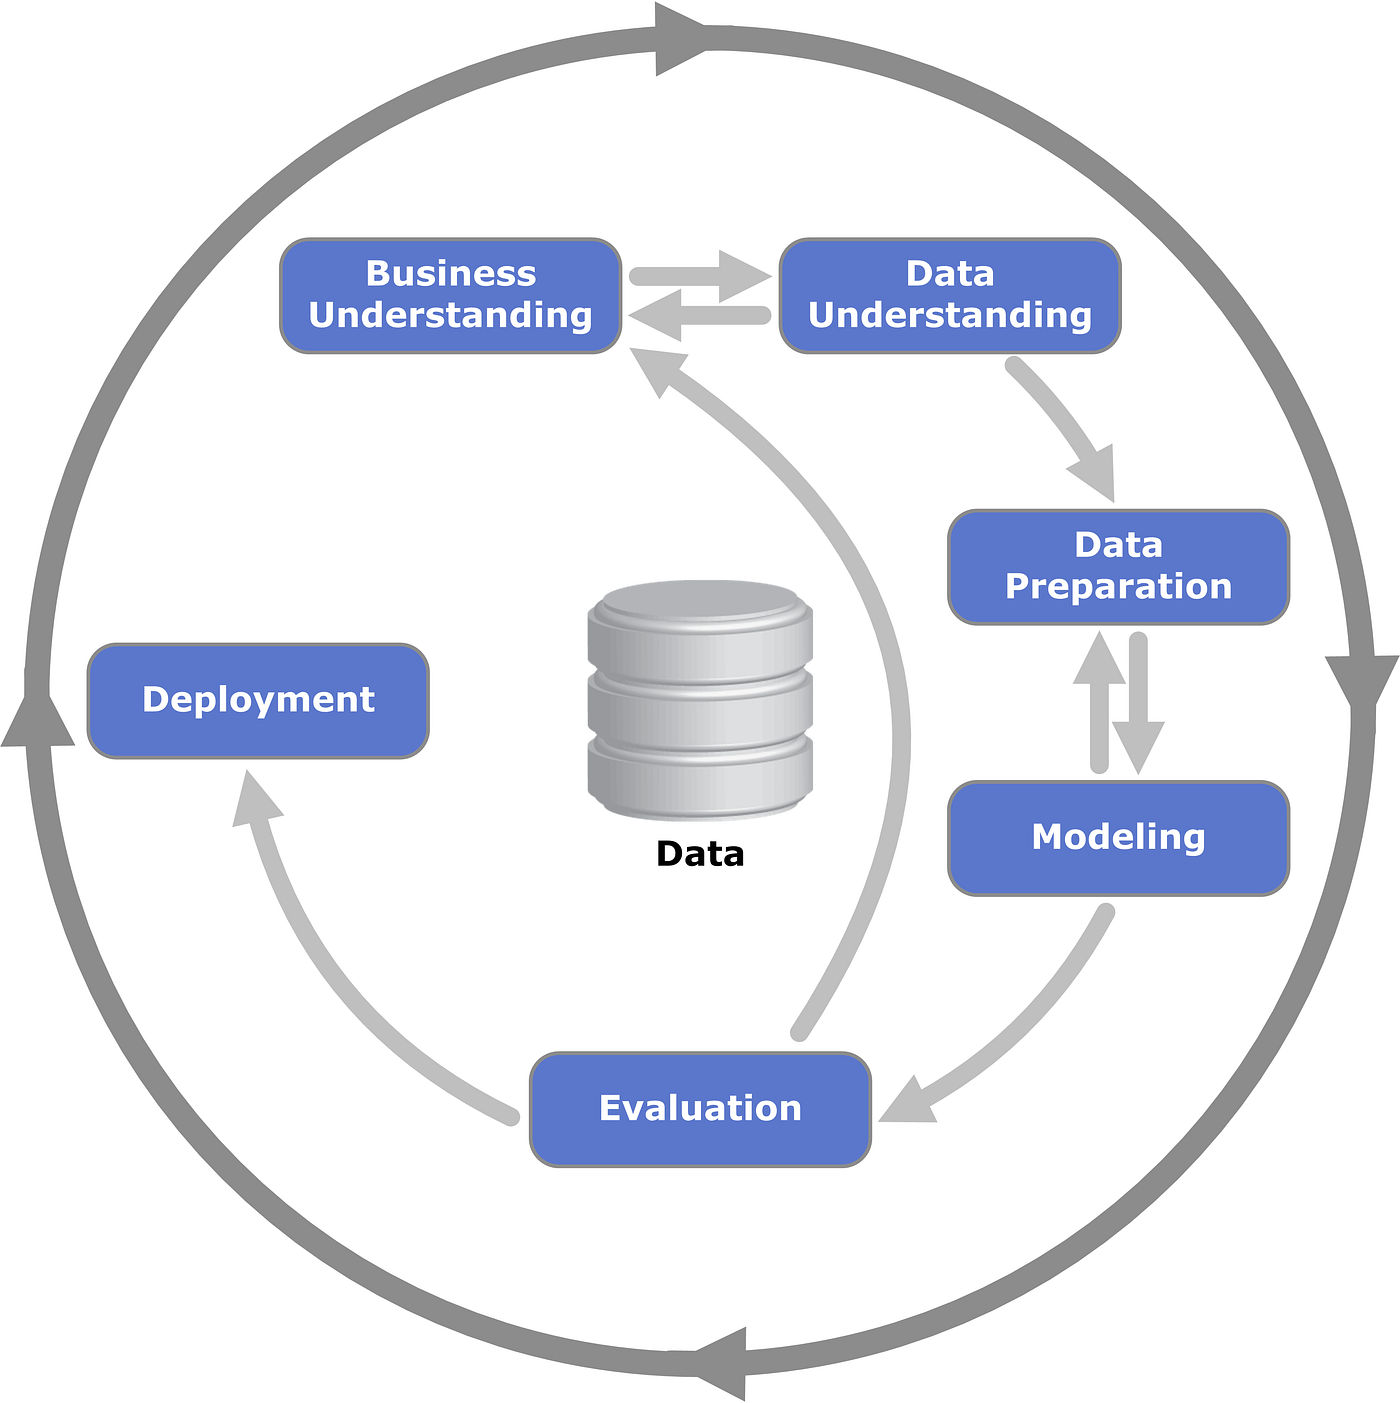
\includegraphics[width=0.4\textwidth]{Gambar/CRISP-DM.png}
    \caption{Alur Kerja CRISP-DM}
    \label{fig:crisp-dm2}
\end{figure}

Gambar \ref{fig:crisp-dm2} menggambarkan alur kerja CRISP-DM yang terdiri dari enam fase utama, yaitu:
\begin{enumerate}
    \item Business Understanding: Memahami tujuan bisnis dan kebutuhan proyek.
    \item Data Understanding: Mengumpulkan dan memahami data yang tersedia.
    \item Data Preparation: Membersihkan dan mempersiapkan data untuk analisis.
    \item Modeling: Membangun model prediktif menggunakan teknik machine learning.
    \item Evaluation: Mengevaluasi model untuk memastikan bahwa tujuan bisnis tercapai.
    \item Deployment: Menerapkan model dalam lingkungan produksi untuk digunakan dalam pengambilan keputusan bisnis.
\end{enumerate}

\subsection{EDA (Exploratory Data Analysis)}
Exploratory Data Analysis (EDA) adalah proses awal dalam analisis data yang bertujuan untuk memahami karakteristik dan pola dalam dataset. EDA melibatkan berbagai teknik visualisasi dan statistik untuk mengeksplorasi data, mengidentifikasi outlier, dan menemukan hubungan antara variabel. Proses ini sangat penting karena membantu dalam mengarahkan langkah-langkah selanjutnya dalam analisis data, seperti pemilihan fitur dan pemodelan. \parencite{tukey1977exploratory}

\subsection{T-Test}
T-Test adalah metode statistik yang digunakan untuk membandingkan rata-rata dari dua kelompok data. Uji ini membantu menentukan apakah perbedaan antara kedua kelompok tersebut signifikan secara statistik atau hanya terjadi secara kebetulan. T-Test dapat digunakan dalam berbagai konteks, seperti membandingkan hasil tes antara dua kelompok siswa atau mengevaluasi efektivitas dua metode pengajaran yang berbeda. Hasil dari uji T-Test memberikan nilai p-value yang digunakan untuk menilai signifikansi perbedaan antara kedua kelompok. \parencite{deveaux2011intro}

%rumus t-test
Rumus untuk menghitung nilai T-Test ($t$) adalah sebagai berikut:
\begin{equation}
    t = \frac{\bar{X_1} - \bar{X_2}}{\sqrt{\frac{s_1^2}{n_1} + \frac{s_2^2}{n_2}}}
\end{equation}
Dimana:
\begin{itemize}
    \item $t$ = nilai T-Test
    \item $\bar{X_1}$ = rata-rata kelompok pertama
    \item $\bar{X_2}$ = rata-rata kelompok kedua
    \item $s_1^2$ = varians kelompok pertama
    \item $s_2^2$ = varians kelompok kedua
    \item $n_1$ = ukuran sampel kelompok pertama
    \item $n_2$ = ukuran sampel kelompok kedua
\end{itemize}

Singkatnya uji t-test ini memudahkan kita dalam membandingkan dua kelompok data untuk menentukan apakah ada perbedaan yang signifikan antara keduanya. Apabila p-value lebih kecil dari tingkat signifikansi (misalnya 0,05), maka kita menolak hipotesis nol dan menyimpulkan bahwa ada perbedaan yang signifikan antara kedua kelompok tersebut. Ini berguna apabila fitur numerik ingin dibandingkan terhadap target kategorikal.


\subsection{Chi Square Test}
Chi Square Test adalah metode statistik yang digunakan untuk menguji hubungan antara dua variabel kategorikal. Uji ini membandingkan frekuensi yang diamati dalam setiap kategori dengan frekuensi yang diharapkan jika tidak ada hubungan antara variabel. Hasil dari uji Chi Square memberikan nilai p-value yang digunakan untuk menentukan apakah hubungan antara variabel tersebut signifikan secara statistik. \parencite{agresti2018statistical}
% \parencite{agresti2018statistical}

%rumus uji chi square
Rumus untuk menghitung nilai Chi Square ($\chi^2$) adalah sebagai berikut:
\begin{equation}
    \chi^2 = \sum \frac{(O_i - E_i)^2}{E_i}
\end{equation}
Dimana:
\begin{itemize}
    \item $\chi^2$ = nilai Chi Square
    \item $O_i$ = frekuensi yang diamati dalam kategori ke-i
    \item $E_i$ = frekuensi yang diharapkan dalam kategori ke-i
    \item $\sum$ = penjumlahan untuk semua kategori
\end{itemize}

Apabila p-value lebih kecil dari tingkat signifikansi (misalnya 0,05), maka kita menolak hipotesis nol dan menyimpulkan bahwa ada hubungan yang signifikan antara kedua variabel tersebut. Ini berguna apabila fitur kategorikal ingin dibandingkan terhadap target kategorikal.
%\parencite{agresti2018statistical}

\subsection{Standard Scaler}
Standard Scaler adalah teknik normalisasi data yang digunakan untuk mengubah fitur numerik sehingga memiliki rata-rata (mean) nol dan standar deviasi (standard deviation) satu. Proses ini membantu dalam mengurangi skala variabilitas antar fitur, sehingga model machine learning dapat belajar lebih efektif. Standard Scaler sangat berguna ketika fitur-fitur dalam dataset memiliki rentang nilai yang berbeda-beda, karena dapat meningkatkan konvergensi dan kinerja model. \parencite{jain2016feature}
%\parencite{jain2016feature}
Rumus untuk menghitung nilai yang telah dinormalisasi ($z$) menggunakan Standard Scaler adalah sebagai berikut:

\begin{equation}
    z = \frac{(X - \mu)}{\sigma}
\end{equation}
Dimana:
\begin{itemize}
    \item $z$ = nilai yang telah dinormalisasi
    \item $X$ = nilai asli dari fitur
    \item $\mu$ = rata-rata (mean) dari fitur
    \item $\sigma$ = standar deviasi (standard deviation) dari fitur
    \item $X - \mu$ = selisih antara nilai asli dan rata-rata
    \item $\frac{(X - \mu)}{\sigma}$ = hasil pembagian selisih dengan standar deviasi
\end{itemize}

Dengan menggunakan Standard Scaler, setiap fitur numerik dalam dataset akan diubah sehingga memiliki distribusi yang seragam, yang pada gilirannya dapat meningkatkan performa model machine learning.

\subsection{Logistic Regression}
Logistic Regression adalah metode statistik yang digunakan untuk memodelkan hubungan antara satu atau lebih variabel independen (fitur) dengan variabel dependen biner (target). Metode ini digunakan untuk memprediksi probabilitas kejadian suatu peristiwa, seperti apakah seorang kandidat akan diterima atau ditolak dalam proses perekrutan. Logistic Regression menggunakan fungsi logit untuk mengubah output linier menjadi probabilitas yang berada dalam rentang 0 hingga 1. \parencite{hosmer2013applied}
%\parencite{hosmer2013applied}
Rumus untuk menghitung probabilitas ($p$) menggunakan Logistic Regression adalah sebagai berikut:
\begin{equation}
    p = \frac{1}{1 + e^{-(\beta_0 + \beta_1X_1 + \beta_2X_2 + ... + \beta_nX_n)}}
\end{equation}

Dimana:
\begin{itemize}
    \item $p$ = probabilitas kejadian (misalnya, kandidat diterima)
    \item $e$ = basis dari logaritma natural (sekitar 2,718)
    \item $\beta_0$ = intercept (konstanta)
    \item $\beta_1, \beta_2, ..., \beta_n$ = koefisien regresi untuk masing-masing fitur
    \item $X_1, X_2, ..., X_n$ = nilai dari fitur-fitur independen
    \item $\beta_0 + \beta_1X_1 + \beta_2X_2 + ... + \beta_nX_n$ = kombinasi linier dari fitur-fitur
\end{itemize}

Logistic Regression sangat berguna dalam berbagai aplikasi, termasuk analisis risiko kredit, diagnosis medis, dan prediksi perilaku konsumen. Dengan kemampuannya untuk memberikan interpretasi yang jelas melalui koefisien regresi, metode ini memungkinkan pemahaman yang lebih baik tentang faktor-faktor yang mempengaruhi keputusan biner.

\subsection{Decision Tree}
Decision Tree adalah algoritma machine learning yang digunakan untuk klasifikasi dan regresi. Algoritma ini bekerja dengan membagi data menjadi subset berdasarkan fitur-fitur tertentu, sehingga membentuk struktur pohon yang terdiri dari simpul (nodes) dan cabang (branches). Setiap simpul mewakili keputusan berdasarkan nilai fitur, sementara cabang menghubungkan simpul-simpul tersebut. Proses pembagian data berlanjut hingga mencapai simpul daun (leaf nodes) yang memberikan prediksi akhir. Decision Tree sangat populer karena kemampuannya untuk menangani data kategorikal dan numerik, serta memberikan interpretasi yang mudah dipahami.

Rumus untuk menghitung impurity menggunakan Gini Index ($G$) adalah sebagai berikut:

\begin{equation}
    G = 1 - \sum_{i=1}^{C} p_i^2
\end{equation}

Dimana:
\begin{itemize}
    \item $G$ = nilai Gini Index
    \item $C$ = jumlah kelas dalam target
    \item $p_i$ = proporsi dari kelas ke-i dalam subset data
    \item $\sum_{i=1}^{C} p_i^2$ = penjumlahan kuadrat proporsi untuk semua kelas
    \item $1 - \sum_{i=1}^{C} p_i^2$ = hasil pengurangan dari 1 dengan penjumlahan kuadrat proporsi
\end{itemize}

Decision Tree sangat berguna dalam berbagai aplikasi, termasuk diagnosis medis, analisis risiko kredit, dan prediksi perilaku konsumen. Dengan kemampuannya untuk memberikan interpretasi yang jelas melalui struktur pohon, metode ini memungkinkan pemahaman yang lebih baik tentang faktor-faktor yang mempengaruhi keputusan klasifikasi.

\subsection{Random Forest}
Random Forest adalah algoritma ensemble learning yang digunakan untuk klasifikasi dan regresi. Algoritma ini bekerja dengan membangun sejumlah besar pohon keputusan (decision trees) secara acak dan menggabungkan hasil prediksi dari masing-masing pohon untuk menghasilkan prediksi akhir yang lebih akurat dan stabil. Random Forest mengurangi risiko overfitting yang sering terjadi pada pohon keputusan tunggal dengan cara mengambil rata-rata (untuk regresi) atau mode (untuk klasifikasi) dari hasil prediksi semua pohon dalam hutan. \parencite{breiman2001random}
%\parencite{breiman2001random}

Rumus untuk menghitung prediksi akhir ($\hat{y}$) dalam Random Forest adalah sebagai berikut:

\begin{equation}
    \hat{y} = \frac{1}{T} \sum_{t=1}^{T} h_t(X)
\end{equation}
Dimana:
\begin{itemize}
    \item $\hat{y}$ = prediksi akhir dari Random Forest
    \item $T$ = jumlah pohon keputusan dalam hutan
    \item $h_t(X)$ = prediksi dari pohon keputusan ke-t untuk input $X$
    \item $\sum_{t=1}^{T} h_t(X)$ = penjumlahan prediksi dari semua pohon keputusan
    \item $\frac{1}{T} \sum_{t=1}^{T} h_t(X)$ = hasil pembagian penjumlahan dengan jumlah pohon untuk mendapatkan rata-rata prediksi
\end{itemize}

Random Forest sangat berguna dalam berbagai aplikasi, termasuk diagnosis medis, analisis risiko kredit, dan prediksi perilaku konsumen. Dengan kemampuannya untuk menangani data yang kompleks dan memberikan interpretasi yang jelas melalui fitur penting (feature importance), metode ini memungkinkan pemahaman yang lebih baik tentang faktor-faktor yang mempengaruhi keputusan klasifikasi atau regresi.

\subsection{XGBoost}
XGBoost (Extreme Gradient Boosting) adalah algoritma machine learning yang digunakan untuk klasifikasi dan regresi. Algoritma ini merupakan implementasi dari teknik boosting yang menggabungkan beberapa model lemah (weak learners), biasanya pohon keputusan, untuk membentuk model yang lebih kuat dan akurat. XGBoost dikenal karena kemampuannya dalam menangani data besar dan kompleks, serta memberikan performa yang tinggi melalui optimasi paralel dan regularisasi.

Rumus untuk menghitung prediksi akhir ($\hat{y}$) dalam XGBoost adalah sebagai berikut:
\begin{equation}
    \hat{y} = \sum_{k=1}^{K} f_k(X)
\end{equation}

Dimana:
\begin{itemize}
    \item $\hat{y}$ = prediksi akhir dari XGBoost
    \item $K$ = jumlah model lemah (pohon keputusan) yang digabungkan
    \item $f_k(X)$ = prediksi dari model lemah ke-k untuk input $X$
    \item $\sum_{k=1}^{K} f_k(X)$ = penjumlahan prediksi dari semua model lemah
\end{itemize}

XGBoost sangat berguna dalam berbagai aplikasi, termasuk diagnosis medis, analisis risiko kredit, dan prediksi perilaku konsumen. Dengan kemampuannya untuk menangani data yang kompleks dan memberikan interpretasi yang jelas melalui fitur penting (feature importance), metode ini memungkinkan pemahaman yang lebih baik tentang faktor-faktor yang mempengaruhi keputusan klasifikasi atau regresi.

\subsection{Confusion Matrix}
Confusion Matrix adalah alat evaluasi yang digunakan untuk menilai kinerja model klasifikasi. Matriks ini menyajikan hasil prediksi model dalam bentuk tabel yang menunjukkan jumlah prediksi benar dan salah untuk setiap kelas. Confusion Matrix terdiri dari empat komponen utama: True Positive (TP), True Negative (TN), False Positive (FP), dan False Negative (FN). Dengan menggunakan Confusion Matrix, kita dapat menghitung berbagai metrik evaluasi seperti akurasi, presisi, recall, dan F1-score, yang memberikan gambaran lebih lengkap tentang kinerja model. Gambar \ref{fig:confusion-matrix} menunjukkan struktur dasar dari Confusion Matrix.\parencite{han2012data}

\begin{figure}[H]
    \centering
    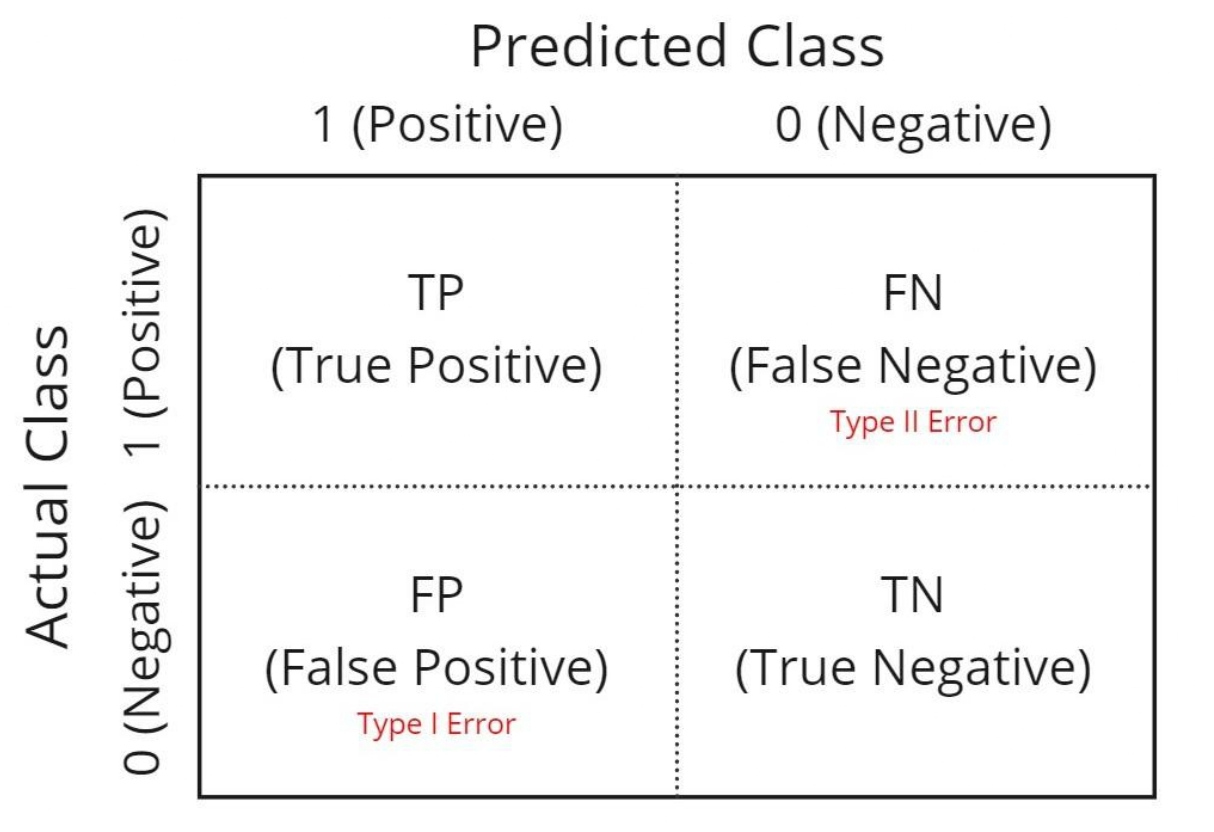
\includegraphics[width=0.5\textwidth]{Gambar/conf.jpg}
    \caption{Struktur Confusion Matrix}
    \label{fig:confusion-matrix}
\end{figure}

Confusion matrix memberikan informasi tentang jumlah prediksi yang benar dan salah untuk setiap kelas. Dari confusion matrix, kita dapat menghitung berbagai metrik evaluasi model seperti akurasi, presisi, recall, dan F1-score. Metrik-metrik ini membantu dalam menilai kinerja model klasifikasi secara keseluruhan.

\subsection{Akurasi}
Akurasi adalah metrik evaluasi yang digunakan untuk mengukur seberapa baik model klasifikasi dalam memprediksi kelas yang benar. Akurasi dihitung sebagai rasio antara jumlah prediksi yang benar (baik True Positive maupun True Negative) dengan total jumlah prediksi yang dibuat oleh model. Metrik ini memberikan gambaran umum tentang kinerja model, namun perlu diingat bahwa akurasi saja tidak selalu mencerminkan kinerja model secara menyeluruh, terutama pada dataset yang tidak seimbang. Oleh karena itu, akurasi sering digunakan bersama dengan metrik lain seperti presisi, recall, dan F1-score untuk mendapatkan evaluasi yang lebih komprehensif. \parencite{jain2016feature}

Rumus untuk menghitung akurasi ($A$) adalah sebagai berikut:
\begin{equation}
    A = \frac{TP + TN}{TP + TN + FP + FN}
\end{equation}
Dimana:
\begin{itemize}
    \item $A$ = akurasi
    \item $TP$ = True Positive (jumlah prediksi benar untuk kelas positif)
    \item $TN$ = True Negative (jumlah prediksi benar untuk kelas negatif)
    \item $FP$ = False Positive (jumlah prediksi salah untuk kelas positif)
    \item $FN$ = False Negative (jumlah prediksi salah untuk kelas negatif)
    \item $TP + TN$ = total prediksi yang benar
    \item $TP + TN + FP + FN$ = total prediksi yang dibuat oleh model
    \item $\frac{TP + TN}{TP + TN + FP + FN}$ = hasil pembagian total prediksi benar dengan total prediksi
\end{itemize}

Akurasi memberikan informasi tentang seberapa sering model membuat prediksi yang benar. Nilai akurasi berkisar antara 0 hingga 1, dimana nilai 1 menunjukkan bahwa model membuat prediksi yang benar untuk semua kasus, sedangkan nilai 0 menunjukkan bahwa model tidak pernah membuat prediksi yang benar. Meskipun akurasi adalah metrik yang berguna, penting untuk mempertimbangkan konteks dan karakteristik dataset saat menilai kinerja model.

\subsection{Presisi}
Presisi adalah metrik evaluasi yang digunakan untuk mengukur seberapa akurat model klasifikasi dalam memprediksi kelas positif. Presisi dihitung sebagai rasio antara jumlah prediksi benar untuk kelas positif (True Positive) dengan total jumlah prediksi yang dibuat untuk kelas positif (True Positive + False Positive). Metrik ini sangat penting dalam situasi di mana biaya kesalahan positif (False Positive) tinggi, seperti dalam diagnosis medis atau deteksi penipuan. Dengan demikian, presisi memberikan gambaran tentang kualitas prediksi model dalam mengidentifikasi kasus positif. \parencite{jain2016feature}

Rumus untuk menghitung presisi ($P$) adalah sebagai berikut:
\begin{equation}
    P = \frac{TP}{TP + FP}
\end{equation}

Dimana:
\begin{itemize}
    \item $P$ = presisi
    \item $TP$ = True Positive (jumlah prediksi benar untuk kelas positif)
    \item $FP$ = False Positive (jumlah prediksi salah untuk kelas positif)
    \item $TP + FP$ = total prediksi yang dibuat untuk kelas positif
    \item $\frac{TP}{TP + FP}$ = hasil pembagian jumlah prediksi benar untuk kelas positif dengan total prediksi untuk kelas positif
\end{itemize}

\subsection{Recall}
Recall adalah metrik evaluasi yang digunakan untuk mengukur seberapa baik model klasifikasi dalam mengidentifikasi semua kasus positif yang sebenarnya. Recall dihitung sebagai rasio antara jumlah prediksi benar untuk kelas positif (True Positive) dengan total jumlah kasus positif yang sebenarnya (True Positive + False Negative). Metrik ini sangat penting dalam situasi di mana biaya kesalahan negatif (False Negative) tinggi, seperti dalam diagnosis medis atau deteksi penipuan. Dengan demikian, recall memberikan gambaran tentang kemampuan model dalam menangkap semua kasus positif yang ada. \parencite{jain2016feature}

Rumus untuk menghitung recall ($R$) adalah sebagai berikut:
\begin{equation}
    R = \frac{TP}{TP + FN}
\end{equation}

Dimana:
\begin{itemize}
    \item $R$ = recall
    \item $TP$ = True Positive (jumlah prediksi benar untuk kelas positif)
    \item $FN$ = False Negative (jumlah prediksi salah untuk kelas negatif)
    \item $TP + FN$ = total kasus positif yang sebenarnya
    \item $\frac{TP}{TP + FN}$ = hasil pembagian jumlah prediksi benar untuk kelas positif dengan total kasus positif yang sebenarnya
    \item $0 \leq R \leq 1$ = nilai recall berkisar antara 0 hingga 1
\end{itemize}

\subsection{F1-Score}
F1-Score adalah metrik evaluasi yang digunakan untuk mengukur keseimbangan antara presisi dan recall dalam model klasifikasi. F1-Score dihitung sebagai rata-rata harmonis dari presisi dan recall, yang memberikan gambaran lebih komprehensif tentang kinerja model, terutama dalam situasi di mana terdapat ketidakseimbangan kelas. Metrik ini sangat berguna ketika kita ingin memastikan bahwa model tidak hanya akurat dalam memprediksi kelas positif, tetapi juga mampu menangkap semua kasus positif yang sebenarnya. \parencite{jain2016feature}

Rumus untuk menghitung F1-Score ($F1$) adalah sebagai berikut:
\begin{equation}
    F1 = 2 \times \frac{P \times R}{P + R}
\end{equation}
Dimana:
\begin{itemize}
    \item $F1$ = F1-Score
    \item $P$ = presisi
    \item $R$ = recall
    \item $P \times R$ = hasil perkalian antara presisi dan recall
    \item $P + R$ = hasil penjumlahan antara presisi dan recall
    \item $2 \times \frac{P \times R}{P + R}$ = hasil perkalian 2 dengan rasio antara hasil perkalian presisi dan recall dengan hasil penjumlahan presisi dan recall
    \item $0 \leq F1 \leq 1$ = nilai F1-Score berkisar antara 0 hingga 1
\end{itemize}

F1-Score memberikan informasi tentang keseimbangan antara presisi dan recall. Nilai F1-Score berkisar antara 0 hingga 1, dimana nilai 1 menunjukkan bahwa model memiliki presisi dan recall yang sempurna, sedangkan nilai 0 menunjukkan bahwa model tidak memiliki presisi atau recall sama sekali. Dengan menggunakan F1-Score, kita dapat menilai kinerja model klasifikasi secara lebih menyeluruh, terutama dalam konteks dataset yang tidak seimbang.

\subsection{ROC-AUC}
ROC-AUC (Receiver Operating Characteristic - Area Under the Curve) adalah metrik evaluasi yang digunakan untuk menilai kinerja model klasifikasi biner. ROC curve adalah grafik yang menunjukkan hubungan antara True Positive Rate (TPR) dan False Positive Rate (FPR) pada berbagai threshold prediksi. AUC adalah luas di bawah kurva ROC, yang memberikan gambaran tentang kemampuan model dalam membedakan antara kelas positif dan negatif. Nilai AUC berkisar antara 0 hingga 1, dimana nilai 1 menunjukkan bahwa model memiliki kemampuan prediksi yang sempurna, sedangkan nilai 0,5 menunjukkan bahwa model tidak lebih baik dari tebakan acak. \parencite{fawcett2006introduction}
Rumus untuk menghitung True Positive Rate (TPR) dan False Positive Rate (FPR) adalah sebagai berikut:
\begin{equation}
    TPR = \frac{TP}{TP + FN}
\end{equation}
\begin{equation}
    FPR = \frac{FP}{FP + TN}
\end{equation}
Dimana:
\begin{itemize}
    \item $TPR$ = True Positive Rate (rasio prediksi benar untuk kelas positif)
    \item $FPR$ = False Positive Rate (rasio prediksi salah untuk kelas positif)
    \item $TP$ = True Positive (jumlah prediksi benar untuk kelas positif)
    \item $FN$ = False Negative (jumlah prediksi salah untuk kelas negatif)
    \item $FP$ = False Positive (jumlah prediksi salah untuk kelas positif)
    \item $TN$ = True Negative (jumlah prediksi benar untuk kelas negatif)
    \item $TP + FN$ = total kasus positif yang sebenarnya
    \item $FP + TN$ = total kasus negatif yang sebenarnya
    \item $\frac{TP}{TP + FN}$ = hasil pembagian jumlah prediksi benar untuk kelas positif dengan total kasus positif yang sebenarnya
    \item $\frac{FP}{FP + TN}$ = hasil pembagian jumlah prediksi salah untuk kelas positif dengan total kasus negatif yang sebenarnya
\end{itemize}

ROC-AUC memberikan informasi tentang kemampuan model dalam membedakan antara kelas positif dan negatif. Nilai AUC berkisar antara 0 hingga 1, dimana nilai 1 menunjukkan bahwa model memiliki kemampuan prediksi yang sempurna, sedangkan nilai 0,5 menunjukkan bahwa model tidak lebih baik dari tebakan acak. Dengan menggunakan ROC-AUC, kita dapat menilai kinerja model klasifikasi secara lebih menyeluruh, terutama dalam konteks dataset yang tidak seimbang.

\subsection{Hyperparameter Tuning}
Hyperparameter tuning adalah proses mengoptimalkan parameter-parameter yang tidak dipelajari oleh model selama pelatihan, tetapi memiliki dampak signifikan terhadap kinerja model. Hyperparameter ini dapat mencakup berbagai aspek seperti jumlah pohon dalam Random Forest, laju pembelajaran (learning rate) dalam XGBoost, atau jumlah iterasi dalam algoritma boosting. Proses tuning melibatkan pencarian kombinasi hyperparameter yang menghasilkan kinerja terbaik pada data validasi, sering kali menggunakan teknik seperti grid search atau random search. Dengan melakukan hyperparameter tuning, kita dapat meningkatkan akurasi dan generalisasi model, sehingga menghasilkan prediksi yang lebih andal pada data baru. \parencite{bergstra2012random}

\subsection{Cross Validation}
Cross Validation adalah teknik evaluasi model yang digunakan untuk menilai kinerja model machine learning dengan membagi dataset menjadi beberapa subset (folds). Proses ini melibatkan pelatihan model pada beberapa subset data dan menguji kinerjanya pada subset yang tersisa. Salah satu metode Cross Validation yang paling umum adalah K-Fold Cross Validation, dimana dataset dibagi menjadi K bagian yang sama, dan model dilatih dan diuji K kali, masing-masing kali menggunakan satu bagian sebagai data uji dan sisanya sebagai data latih. Teknik ini membantu dalam mengurangi overfitting dan memberikan estimasi kinerja model yang lebih akurat dan stabil. \parencite{arlot2010survey}

\subsection{Feature Importance}
Feature Importance adalah teknik yang digunakan untuk mengukur kontribusi masing-masing fitur dalam mempengaruhi prediksi model machine learning. Dengan mengetahui fitur mana yang paling penting, kita dapat memahami faktor-faktor yang paling berpengaruh terhadap hasil prediksi, serta melakukan seleksi fitur untuk meningkatkan kinerja model. Beberapa algoritma, seperti Random Forest dan XGBoost, secara otomatis menghitung feature importance berdasarkan seberapa sering dan seberapa efektif fitur tersebut digunakan dalam pembentukan pohon keputusan.\parencite{molnar2020interpretable}

\subsection{SHAP Values (Shapley Additive Explanations)}
SHAP Values (Shapley Additive Explanations) adalah metode interpretasi model machine learning yang didasarkan pada teori permainan. SHAP Values memberikan penjelasan tentang kontribusi masing-masing fitur terhadap prediksi individu dengan menghitung nilai Shapley, yang merupakan rata-rata kontribusi marginal dari fitur tersebut di semua kemungkinan kombinasi fitur. Metode ini memungkinkan kita untuk memahami bagaimana setiap fitur mempengaruhi hasil prediksi, baik secara positif maupun negatif, sehingga memberikan wawasan yang lebih mendalam tentang perilaku model. SHAP Values sangat berguna dalam konteks model yang kompleks dan sulit diinterpretasikan, seperti ensemble models atau deep learning. \parencite{lundberg2017unified}










